\documentclass[aspectratio=169,11pt]{beamer}

% Packages
\usepackage[utf8]{inputenc}
\usepackage[T1]{fontenc}
\usepackage{lmodern}
\usepackage{microtype}
\usepackage{amsmath,amssymb}
\usepackage{booktabs}
\usepackage{graphicx}
\usepackage{tikz}
\usepackage{pgfplots}
\usepackage{xcolor}
\usepackage{ragged2e}
\usepackage{colortbl}
\usepackage{array}
\usepackage{hyperref}
\usepackage{adjustbox}

\usetikzlibrary{shapes.geometric, arrows.meta, positioning, calc, backgrounds, decorations.pathreplacing, shadows, fadings}
\pgfplotsset{compat=1.18}

% --- Color Palette: Warm Professional ---
\definecolor{DeepNavy}{HTML}{2E4057}
\definecolor{Teal}{HTML}{048A81}
\definecolor{WarmOrange}{HTML}{E85D04}
\definecolor{SoftPurple}{HTML}{9D4EDD}
\definecolor{WarmGray}{HTML}{6C757D}
\definecolor{LightGray}{HTML}{E9ECEF}
\definecolor{Cream}{HTML}{FBF8F1}
\definecolor{DeepRed}{HTML}{D62828}
\definecolor{Gold}{HTML}{D4A03A}
\definecolor{SoftWhite}{HTML}{FAFAFA}

% Beamer colors
\setbeamercolor{normal text}{fg=DeepNavy, bg=SoftWhite}
\setbeamercolor{structure}{fg=DeepNavy}
\setbeamercolor{alerted text}{fg=DeepRed}
\setbeamercolor{example text}{fg=Teal}
\setbeamercolor{frametitle}{fg=DeepNavy, bg=SoftWhite}
\setbeamercolor{title}{fg=DeepNavy}
\setbeamercolor{subtitle}{fg=WarmGray}
\setbeamercolor{block title}{bg=DeepNavy, fg=SoftWhite}
\setbeamercolor{block body}{bg=LightGray, fg=DeepNavy}
\setbeamercolor{itemize item}{fg=WarmOrange}
\setbeamercolor{itemize subitem}{fg=Gold}

% Fonts
\usefonttheme{professionalfonts}
\setbeamerfont{title}{size=\huge, series=\bfseries}
\setbeamerfont{frametitle}{size=\Large, series=\bfseries}

% Strip chrome
\setbeamertemplate{navigation symbols}{}
\setbeamertemplate{headline}{}

% Minimal footline
\setbeamertemplate{footline}{%
    \hfill
    \begin{beamercolorbox}[wd=3cm,ht=2.5ex,dp=1ex,right,rightskip=0.6cm]{page number}
        \usebeamercolor[fg]{WarmGray}\scriptsize\insertframenumber
    \end{beamercolorbox}
    \vspace{0.3cm}
}

% Bullets
\setbeamertemplate{itemize item}{\footnotesize\raisebox{0.3ex}{\tikz\fill[WarmOrange] (0,0) circle (0.45ex);}}
\setbeamertemplate{itemize subitem}{\footnotesize\raisebox{0.3ex}{\tikz\fill[Gold] (0,0) circle (0.35ex);}}

% Custom commands
\newcommand{\transitionslide}[2]{%
    {\setbeamercolor{normal text}{fg=SoftWhite,bg=DeepNavy}
    \begin{frame}[plain]\vfill\begin{center}
        {\huge\bfseries\textcolor{Gold}{#1}}\\[0.6cm]
        {\large\textcolor{LightGray}{#2}}
    \end{center}\vfill\end{frame}}
}

\begin{document}

\begin{frame}
    \title{Granular Instrumental Variables}
    \subtitle{Gabaix and Koijen (2022)}
    \author{Roy Kisluk}
    \date{\today}
    \titlepage
\end{frame}


%%%%%%%%%%%%%%%%%%%%%%%%%%%%%%%%%%%%%%%%%%%%%%%%%%%%%%%%%%%%%%%%%%%%%%%%%%%%%%%%
% Introduction

\begin{frame}
    \frametitle{Endogenous aggregate shocks confound the effect of large firms}

    \vspace{0.5cm}
    {\Large
        The Goal: Estimate the causal elasticity of wages to labor demand.
    }

    \vspace{0.8cm}
    {\Large
        The Identification Challenge: \textbf{Simultaneity}
    }

    \vspace{0.4cm}
    \begin{itemize}
        \item \textbf{Supply Equation:} Wages respond to labor demand and macro supply shocks.
        \item \textbf{Demand Equation:} Labor demand responds to wages and macro demand shocks.
    \end{itemize}


\end{frame}

\begin{frame} \label{src_sqrtn}
    \frametitle{The Law of Large Numbers fails in modern economies}
    \begin{columns}[T]
        \begin{column}{0.55\textwidth}


            \vspace{0.8cm}
            \begin{enumerate}
                \item {In a standard economy, micro-shocks cancel out at a rate of $1/\sqrt{N}$ \hyperlink{app_sqrtn}{\beamergotobutton{Proof}}
                      \vspace{0.4cm}}
                \item {In a \textbf{granular} economy, where the size distribution of firms follows a power law (i.e., Zipf's Law: $\text{size} \propto \frac{1}{\text{rank}}$), a few firms are so large that their idiosyncratic luck drives aggregate volatility.}
            \end{enumerate}
        \end{column}

        \begin{column}{0.45\textwidth}
            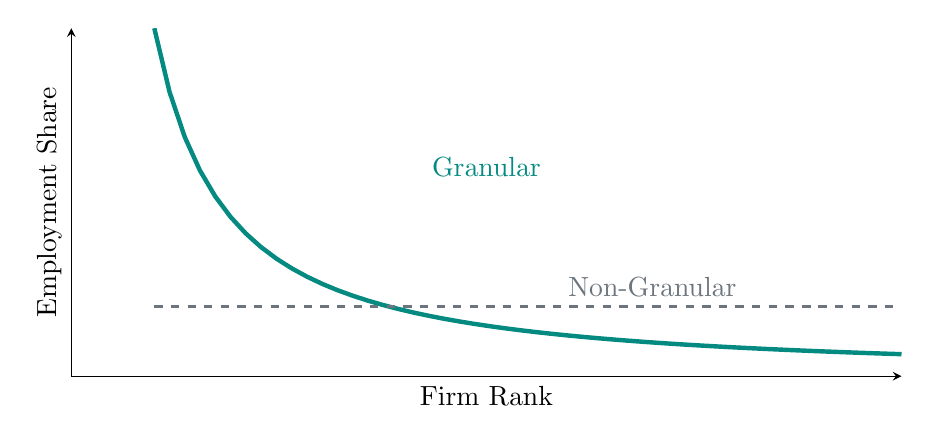
\begin{tikzpicture}
                \begin{axis}[
                        width=\textwidth, height=6cm,
                        axis lines=left,
                        xlabel={Firm Rank},
                        ylabel={Employment Share},
                        xmin=0, xmax=10,
                        ymin=0, ymax=1,
                        ticks=none
                    ]
                    \addplot[Teal, ultra thick, domain=1:10, samples=50] {1/x^1.2};
                    \node[Teal] at (axis cs: 5, 0.6) {Granular};

                    \addplot[WarmGray, thick, dashed, domain=1:10, samples=50] {0.2};
                    \node[WarmGray, anchor=south] at (axis cs: 7, 0.2) {Non-Granular};
                \end{axis}
            \end{tikzpicture}
        \end{column}
    \end{columns}

\end{frame}


%%%%%%%%%%%%%%%%%%%%%%%%%%%%%%%%%%%%%%%%%%%%%%%%%%%%%%%%%%%%%%%%%%%%%%%%%%%%%%%%
% THE SIMPLE MODEL
\transitionslide{A Simple Model}{}
\begin{frame} \label{src_assumptions}
    \frametitle{A simple model of aggregate and idiosyncratic shocks}

    Consider an economy with $N$ firms. The system is given by:



    \begin{align}
        w_t    & = \psi L_{St} + \varepsilon_t \tag{Supply}  \\[0.5cm]
        L_{it} & = \phi^d w_t + \eta_t + u_{it} \tag{Demand}
    \end{align}

    Where:
    \begin{itemize}
        \item $w_t$ is the wage (observed)
        \item $L_{it}$ is the number of workers at firm $i$ (observed)
        \item $\eta_t$ and $\varepsilon_t$ are aggregate shocks (unobserved)
        \item $u_{it}$ is the idiosyncratic shock to firm $i$ (unobserved)
        \item Main assumption: $u_{it}$ are uncorrelated with aggregate shocks ($\eta_t, \epsilon_t$) \hyperlink{app_assumptions}{\beamergotobutton{Assumptions}}
    \end{itemize}
    \vspace{0.2cm}
    We cannot estimate $\psi$ (labor supply elasticity) and $\phi^d$ (labor demand elasticity) by OLS, due to simultaneity.
\end{frame}



\begin{frame}
    \frametitle{Constructing the Granular Instrumental Variable ($z_t$)}

    {
        The GIV exploits the difference between size-weighted and equal-weighted averages.
    }

    \vspace{0.2cm}
    Define the equal-weighted average outcome:
    \begin{equation*}
        L_{Et} = \frac{1}{N} \sum_{i=1}^N L_{it} \tag{Equal-Weighted Average}
    \end{equation*}
    Define the size-weighted average outcome:
    \begin{equation*}
        L_{St} = \sum_{i=1}^N S_i L_{it}, \quad \sum_{i=1}^N S_i = 1 \tag{Size-Weighted Average}
    \end{equation*}

    \vspace{0.5cm}
    The GIV is the size-weighted outcome minus the equal-weighted outcome:
    \begin{equation}
        z_t := L_{\Gamma t} = L_{St} - L_{Et} \tag{GIV}
    \end{equation}

\end{frame}

\begin{frame} \label{src_equal_weighted}
    \frametitle{The GIV isolates purely idiosyncratic firm shocks}

    \vspace{0.5cm}
    Substitute the demand equation into the aggregate definitions: \hyperlink{app_size_weighted}{\beamergotobutton{Proof}}
    \begin{align}
        L_{St} & = \phi^d w_t + \eta_t + u_{St} \notag \\
        L_{Et} & = \phi^d w_t + \eta_t + u_{Et} \notag
    \end{align}

    \vspace{0.5cm}
    The common components ($\phi^d w_t + \eta_t$) difference out:
    \begin{equation}
        z_t = u_{\Gamma t} = u_{St} - u_{Et} = \sum_{i=1}^N S_i u_{it} - \frac{1}{N} \sum_{i=1}^N u_{it} = \sum_{i=1}^N (S_i - \frac{1}{N}) u_{it} \tag{GIV}
    \end{equation}

    \vspace{0.5cm}
    {\Large
        $z_t$ is made \emph{only} of idiosyncratic shocks.
    }

\end{frame}

\begin{frame}
    \frametitle{GIV estimates elasticities via 2SLS}
    \begin{itemize}
        \item \large{\textbf{First Stage:} Regress aggregate labor demand ($L_{St}$) on the granular instrument ($z_t$). This extracts $\widehat{L}_{St}$, the variation driven \emph{only} by the idiosyncratic shocks of firms.}
              % \begin{equation*}
              %     L_{St} = \beta z_t + \text{Controls} + \nu_t
              % \end{equation*}
              \vspace{0.5cm}
        \item \large{\textbf{Second Stage:} Regress aggregate wages ($w_t$) on the predicted labor demand from the First Stage ($\widehat{L}_{St}$) to obtain an unbiased estimate of $\psi$.}
              % \begin{equation*}
              %     w_t = \psi \widehat{L}_{St} + \text{Controls} + \varepsilon_t
              % \end{equation*}
    \end{itemize}

\end{frame}

\begin{frame}
    \frametitle{Validating the Instrument: Relevance and Exclusion}

    \vspace{0.3cm}
    {\Large
        For $z_t$ to be a valid instrument, two fundamental assumptions must hold in a granular economy.
    }

    \vspace{0.8cm}
    \begin{itemize}
        \item \textbf{Relevance ($\text{Cov}(L_{St}, z_t) \neq 0$):}\\
              \vspace{0.2cm}
              The granular shocks must actually move the aggregate market. This requires a \emph{concentrated market} (e.g., high Herfindahl index) where the idiosyncratic shocks of the largest firms are volatile enough to shift total labor demand.

              \vspace{0.6cm}
        \item \textbf{Exclusion Restriction ($\text{Cov}(z_t, \varepsilon_t) = 0$, $\text{Cov}(z_t, \eta_t) = 0$):}\\
              \vspace{0.2cm}
              The idiosyncratic shocks of large firms ($z_t$) must not directly affect aggregate wages ($w_t$) through any channel other than aggregate labor demand ($L_{St}$). They must be truly orthogonal to macro aggregate supply shocks ($z_t \perp \eta_t, \varepsilon_t$).
    \end{itemize}

\end{frame}

\begin{frame} \label{src_psi_identification}
    \frametitle{The GIV yields both supply and demand elasticities}

    \vspace{0.5cm}
    By exogeneity, $\mathbb{E}[u_t \varepsilon_t] = 0 \implies \mathbb{E}[z_t \varepsilon_t] = 0$, where $u_t = (u_{it})_{i=1,\dots,N}$.

    \vspace{0.5cm}
    Using the supply equation:
    \begin{equation*}
        w_t = \psi L_{St} + \varepsilon_t \quad \implies \quad \mathbb{E}[(w_t - \psi L_{St}) z_t] = 0
    \end{equation*}
    \begin{equation*}
        \psi = \frac{\mathbb{E}[w_t z_t]}{\mathbb{E}[L_{St} z_t]} \tag{Supply Elasticity}
    \end{equation*}
    \hyperlink{app_psi_identification}{\beamergotobutton{Proof}}

    \vspace{0.5cm}
    Using the equal-weighted demand equation, $\mathbb{E}[(L_{Et} - \phi^d w_t) z_t] = 0$:
    \begin{equation*}
        \phi^d = \frac{\mathbb{E}[L_{Et} z_t]}{\mathbb{E}[w_t z_t]} \tag{Demand Elasticity}
    \end{equation*}

\end{frame}

%%%%%%%%%%%%%%%%%%%%%%%%%%%%%%%%%%%%%%%%%%%%%%%%%%%%%%%%%%%%%%%%%%%%%%%%%%%%%%%%
% THE FULL MODEL
\transitionslide{The Full Model}{Handling heterogeneous factor loadings}


\begin{frame} \label{src_simple_giv_fails}
    \frametitle{The Full Factor Model for granular firms}
    We now allow for heterogeneous loadings $\lambda_i$:
    \begin{equation}
        L_{it} = \phi w_t + \lambda_i \eta_t + u_{it} \notag
    \end{equation}
    The simple GIV ($L_{St} - L_{Et}$) assumes every firm has the same loading $\lambda_i = 1$.
    If large firms are more sensitive to the Fed, the simple GIV is \textbf{"leaky"}—it correlates with $\eta_t$.\\[0.4cm]
    The simple GIV becomes: \hyperlink{app_simple_giv_fails}{\beamergotobutton{Proof}}
    \begin{equation*}
        z_t = (\lambda_S - \lambda_E) \eta_t + (u_{St} - u_{Et})
    \end{equation*}
    {
    If $\lambda_S \neq \lambda_E$, the instrument is \textbf{invalid} ($\mathbb{E}[z_t \eta_t] \neq 0$, i.e., the Exclusion Restriction fails).
    }
\end{frame}



\begin{frame}
    \frametitle{The Solution: Orthogonal Optimal Weights $\Gamma$}
    Substitute Equation $L_{it} = \phi w_t + \lambda_i \eta_t + u_{it}$ into the definition of the weighted GIV:
    \begin{align*}
        z_t & = \sum \Gamma_i L_{it} = \sum \Gamma_i (\phi w_t + \lambda_i \eta_t + u_{it})        \\
            & = \phi w_t (\sum \Gamma_i) + \eta_t (\sum \Gamma_i \lambda_i) + \sum \Gamma_i u_{it}
    \end{align*}
    Where $\Gamma$ is the vector of weights that we want to find.\\
    To ensure $z_t$ contains \textit{only} idiosyncratic shocks ($u_{it}$), we must satisfy two conditions:
    \begin{enumerate}
        \item $\sum \Gamma_i = 0$: This removes the endogenous wage $w_t$.
        \item $\sum \Gamma_i \lambda_i = 0$: This removes the common macro shock $\eta_t$.
    \end{enumerate}
    We need weights $\Gamma$ such that the factor components \textbf{cancel exactly}.
    This ensures $z_t = \sum \Gamma_i u_{it}$ is purely idiosyncratic.


\end{frame}

\begin{frame} \label{src_propositions}
    \frametitle{Choosing Optimal Weights $\Gamma$}
    For this, we use the $N \times N$ projection matrix $Q$ that is orthogonal to the factor loadings—that is, $Q \lambda = 0$: \hyperlink{app_refresher}{\beamergotobutton{Refresher}}
    \begin{equation*}
        Q = I - \lambda (\lambda' \lambda)^{-1} \lambda'
    \end{equation*}
    The optimal weights are then given by $\Gamma^{*\prime} = S'Q$. \hyperlink{app_propositions}{\beamergotobutton{Propositions}}
    \begin{itemize}
        \item Intuitively, we want $\Gamma$ to be as close as possible to $S$ but satisfy $\Gamma \perp \lambda$. This is a standard projection problem: $\Gamma = S - \lambda (\lambda' \lambda)^{-1} \lambda' S$
        \item In essence, we take the firm sizes and subtract the portion of size that is explained by macro-sensitivity. What remains is pure granular weight.
    \end{itemize}


\end{frame}


\transitionslide{Application}{GIV in the Israeli Labor Market}

\begin{frame}
    \frametitle{The Israeli Tech Sector is highly granular}

    \vspace{0.5cm}
    {\Large
        The Israeli high-tech industry is dominated by a few massive multinational R\&D centers.
    }

    \vspace{1cm}
    \begin{itemize}
        \item \textbf{High Concentration:} Companies like Intel, Google, Microsoft, and NVIDIA account for a substantial, disproportionate share of tech employment.
        \item \textbf{A Heavy Tail:} The size distribution of tech employers in Israel exhibits a strong power law, yielding a high \textbf{excess Herfindahl index ($h$)}.
        \item \textbf{Macro vs. Micro:} It is difficult to separate general Israeli macroeconomic conditions (e.g., security shocks, interest rates) from the hiring dynamics of these specific giants.
    \end{itemize}
\end{frame}

\begin{frame}
    \frametitle{Applying GIV to Israeli tech wages}

    \vspace{0.5cm}
    {\Large
        How do we isolate the causal spillover of these tech giants on aggregate Israeli wages?
    }

    \vspace{1cm}
    \begin{itemize}
        \item \textbf{The Idiosyncratic Shocks ($u_{it}$):} We exploit global shocks specific to the multinationals that are arguably exogenous to the Israeli macroeconomy (e.g., global restructuring at Intel, a worldwide AI hiring boom at NVIDIA).
        \item \textbf{The Instrument ($z_t$):} Construct the GIV by taking the size-weighted employment shocks of these giants and projecting out the common Israeli macroeconomic factor loadings.
        \item \textbf{The 2SLS Estimation:} Regress aggregate Israeli wages on the component of labor demand driven \emph{only} by these isolated, granular tech shocks.
    \end{itemize}
\end{frame}

\begin{frame}
    \frametitle{Takeaways: GIV unconfounds local macro dynamics}

    \vspace{1cm}
    {\Large
        The GIV method solves the simultaneity problem in concentrated labor markets.
    }

    \vspace{1cm}
    \begin{itemize}
        \item \textbf{Causal Wage Spillovers:} We can measure exactly how much a hiring freeze at a major tech firm depresses aggregate local wages, separated from a general economic downturn.
        \item \textbf{Beyond the US:} The method is perfectly suited for small, open economies like Israel, where granular actors often drive aggregate volatility.
    \end{itemize}
\end{frame}

\transitionslide{Appendix A}{Derivations}

\begin{frame}{Assumptions}
    \label{app_assumptions}
    \vspace{-0.5em}
    \begin{block}{The Central Identification Assumption}
        Individual shocks $u_{it}$ are truly idiosyncratic—uncorrelated with aggregate shocks ($\eta_t, \epsilon_t$) and controls ($C_t^y, C_t^p$):
        \begin{equation}
            u_t \perp \eta_t, \epsilon_t, C_t^y, C_t^p
        \end{equation}
    \end{block}

    \vfill

    \begin{columns}[T]
        \begin{column}{0.48\textwidth}
            \textbf{Baseline Simplifications}
            \begin{description}
                \item[A1] Factor loadings $\lambda_i$ are known (relaxed in §IV.B).
                \item[A2] Controls have factor structure: $C_{it}^y = \lambda_i c_t^y$.
            \end{description}
        \end{column}
        \begin{column}{0.48\textwidth}
            \textbf{Error Structure}
            \begin{description}
                \item[A3] Homoskedastic and uncorrelated across $i$: $\mathbb{E}[u_t u_t'] = \sigma_u^2 I$.
                \item[A4] General heteroskedasticity $V^u$ (relaxed for optimality).
            \end{description}
        \end{column}
    \end{columns}

    \vfill
    \footnotesize
    \textit{Note: All random variables are assumed to have finite fourth moments and are i.i.d. across periods.}
    \vspace{0.1cm}
    \hfill \hyperlink{src_assumptions}{\beamerreturnbutton{Back}}
\end{frame}

\begin{frame}
    \label{app_sqrtn}
    \frametitle{Aggregate volatility decays at $1/\sqrt{N}$ under equal weights}

    \vspace{0.4cm}
    Suppose there are $N$ firms, each receiving an independent idiosyncratic shock $u_{it}$.
    Assume these shocks have mean 0 and a common variance $\sigma^2$:
    \begin{equation*}
        \mathbb{E}[u_{it}] = 0, \quad \text{Var}(u_{it}) = \sigma^2, \quad \text{Cov}(u_{it}, u_{jt}) = 0 \text{ for } i \neq j
    \end{equation*}

    \vspace{0.4cm}
    In a non-granular economy, the aggregate shock is an \textbf{equal-weighted} average:
    \begin{equation*}
        u_{Et} = \frac{1}{N} \sum_{i=1}^N u_{it}
    \end{equation*}

    \vspace{0.4cm}
    The variance of the aggregate shock is:
    \begin{equation*}
        \text{Var}(u_{Et}) = \text{Var}\left( \frac{1}{N} \sum u_{it} \right) = \frac{1}{N^2} \sum \text{Var}(u_{it}) = \frac{N \sigma^2}{N^2} =
        \frac{\sigma^2}{N}
    \end{equation*}

    {
    The aggregate volatility is therefore: { $\sigma_{agg} = \frac{\sigma}{\sqrt{N}}$}
    }

    \vspace{0.1cm}
    \hfill \hyperlink{src_sqrtn}{\beamerreturnbutton{Back}}
\end{frame}

\begin{frame} \label{app_size_weighted}
    \frametitle{Deriving the Size-Weighted Aggregate ($L_{St}$)}
    The size-weighted outcome is defined as $L_{St} = \sum_{i=1}^N S_i L_{it}$, where $S_i$ are weights such that $\sum S_i = 1$.

    \begin{align*}
        L_{St} & = \sum_{i=1}^N S_i (\phi^d w_t + \eta_t + u_{it})                                 \\
        L_{St} & = \sum_{i=1}^N S_i \phi^d w_t + \sum_{i=1}^N S_i \eta_t + \sum_{i=1}^N S_i u_{it}
    \end{align*}

    Since $\phi^d$, $w_t$, and $\eta_t$ do not depend on the index $i$, we can pull them out:
    \begin{align*}
        L_{St} & = \phi^d w_t \left( \sum_{i=1}^N S_i \right) + \eta_t \left( \sum_{i=1}^N S_i \right) + \sum_{i=1}^N S_i u_{it}
    \end{align*}

    Using the property $\sum S_i = 1$ and defining the size-weighted idiosyncratic shock as $u_{St} = \sum S_i u_{it}$, we get:
    \begin{equation}
        L_{St} = \phi^d w_t + \eta_t + u_{St} \notag
    \end{equation}
    \vspace{0.1cm}
    \hfill \hyperlink{src_equal_weighted}{\beamerreturnbutton{Back}}
\end{frame}

\begin{frame} \label{app_equal_weighted}
    \frametitle{Deriving the Equal-Weighted Aggregate ($L_{Et}$)}
    The equal-weighted outcome is defined as $L_{Et} = \frac{1}{N} \sum_{i=1}^N L_{it}$.

    \begin{align*}
        L_{Et} & = \frac{1}{N} \sum_{i=1}^N (\phi^d w_t + \eta_t + u_{it})                                                 \\
        L_{Et} & = \frac{1}{N} \sum_{i=1}^N \phi^d w_t + \frac{1}{N} \sum_{i=1}^N \eta_t + \frac{1}{N} \sum_{i=1}^N u_{it}
    \end{align*}

    Again, pulling constants out of the summations:
    \begin{align*}
        L_{Et} & = \phi^d w_t \left( \frac{1}{N} \sum_{i=1}^N 1 \right) + \eta_t \left( \frac{1}{N} \sum_{i=1}^N 1 \right) + \frac{1}{N} \sum_{i=1}^N u_{it}
    \end{align*}

    Since $\frac{1}{N} \sum_{i=1}^N 1 = \frac{1}{N} \cdot N = 1$, and defining the equal-weighted idiosyncratic shock as $u_{Et} = \frac{1}{N} \sum u_{it}$, we get:
    \begin{equation}
        L_{Et} = \phi^d w_t + \eta_t + u_{Et} \notag
    \end{equation}
    \vspace{0.1cm}
    \hfill \hyperlink{src_equal_weighted}{\beamerreturnbutton{Back}}
\end{frame}

\begin{frame} \label{app_psi_identification}
    \frametitle{Identifying Supply Elasticity ($\psi$)}
    To find $\psi$, we use $z_t$ as an instrument for $L_{St}$ in the supply equation. We take the expectation of the product of the supply equation and the instrument:
    \begin{align*}
        \mathbb{E}[w_t z_t] & = \mathbb{E}[(\psi L_{St} + \epsilon_t) z_t]               \\
        \mathbb{E}[w_t z_t] & = \psi \mathbb{E}[L_{St} z_t] + \mathbb{E}[\epsilon_t z_t]
    \end{align*}
    By the exogeneity condition, $\mathbb{E}[\epsilon_t z_t] = 0$. Thus:
    \begin{equation}
        \psi = \frac{\mathbb{E}[w_t z_t]}{\mathbb{E}[L_{St} z_t]}
    \end{equation}
    This is the standard IV formula where $z_t$ instruments for $L_{St}$.
    \vspace{0.1cm}
    \hfill \hyperlink{src_psi_identification}{\beamerreturnbutton{Back}}
\end{frame}

\begin{frame}
    \frametitle{Identifying Demand Elasticity ($\phi^d$)}
    To find $\phi^d$, we use the equal-weighted aggregate demand equation derived on slide 8:
    \begin{equation}
        L_{Et} = \phi^d w_t + \eta_t + u_{Et} \tag{41}
    \end{equation}
    We aim to show that $\mathbb{E}[(L_{Et} - \phi^d w_t) z_t] = 0$. Substituting the demand equation:
    \begin{equation}
        \mathbb{E}[(L_{Et} - \phi^d w_t) z_t] = \mathbb{E}[(\eta_t + u_{Et}) z_t] = \mathbb{E}[\eta_t z_t] + \mathbb{E}[u_{Et} z_t]
    \end{equation}
    We already know $\mathbb{E}[\eta_t z_t] = 0$. Now we examine $\mathbb{E}[u_{Et} z_t]$. Under the assumption that $u_{it}$ are i.i.d. with variance $\sigma_u^2$:
    \begin{align*}
        \mathbb{E}[u_{Et} z_t] & = \mathbb{E}[u_{Et} (u_{St} - u_{Et})]             \\
                               & = \mathbb{E}[u_{Et} u_{St}] - \mathbb{E}[u_{Et}^2]
    \end{align*}
    \vspace{0.1cm}
    \hfill \hyperlink{src_psi_identification}{\beamerreturnbutton{Back}}
\end{frame}
\begin{frame}
    \frametitle{Identifying Demand Elasticity ($\phi^d$)}
    \begin{align*}
        \mathbb{E}[u_{Et} u_{St}] - \mathbb{E}[u_{Et}^2]    =
        \\
         & = \mathbb{E} \left[ \left( \frac{1}{N} \sum_{i} u_{it} \right) \left( \sum_{j} S_j u_{jt} \right) \right] - \mathbb{E} \left[ \left( \frac{1}{N} \sum_{i} u_{it} \right)^2 \right] \\
         & = \frac{1}{N} \sum_{i} S_i \sigma_u^2 - \frac{1}{N^2} \sum_{i} \sigma_u^2                                                                                                          \\
         & = \frac{1}{N} \sigma_u^2 (1) - \frac{1}{N} \sigma_u^2 = 0
    \end{align*}
    Since $\mathbb{E}[u_{Et} z_t] = 0$, it follows that $\mathbb{E}[(L_{Et} - \phi^d w_t) z_t] = 0$. Rearranging:
    \begin{align*}
        \mathbb{E}[L_{Et} z_t] & = \phi^d \mathbb{E}[w_t z_t]                         \\
        \phi^d                 & = \frac{\mathbb{E}[L_{Et} z_t]}{\mathbb{E}[w_t z_t]}
    \end{align*}
    \vspace{0.1cm}
    \hfill
\end{frame}

\begin{frame} \label{app_simple_giv_fails}
    \frametitle{Derivation: Why the Simple GIV Fails}
    The simple GIV is defined as $z_t^{simple} = L_{St} - L_{Et}$. Let's derive its components:

    1. \textbf{Size-weighted average ($L_{St}$):}
    \begin{align*}
        L_{St} & = \sum S_i L_{it} = \sum S_i (\phi w_t + \lambda_i \eta_t + u_{it})                                                               \\
               & = \phi w_t \underbrace{\sum S_i}_{1} + \eta_t \underbrace{\sum S_i \lambda_i}_{\lambda_S} + \underbrace{\sum S_i u_{it}}_{u_{St}} \\
               & = \phi w_t + \lambda_S \eta_t + u_{St}
    \end{align*}

    2. \textbf{Equal-weighted average ($L_{Et}$):}
    \begin{align*}
        L_{Et} & = \frac{1}{N} \sum L_{it} = \phi w_t + \eta_t \underbrace{\frac{1}{N} \sum \lambda_i}_{\lambda_E} + u_{Et} \\
               & = \phi w_t + \lambda_E \eta_t + u_{Et}
    \end{align*}

    3. \textbf{The Resulting GIV:} \hyperlink{src_simple_giv_fails}{\beamerreturnbutton{Back}}
    \begin{equation}
        z_t^{simple} = L_{St} - L_{Et} = \mathbf{(\lambda_S - \lambda_E) \eta_t} + (u_{St} - u_{Et}) \notag
    \end{equation}

    \vspace{0.1cm}
    \hfill \hyperlink{src_simple_giv_fails}{\beamerreturnbutton{Back}}
\end{frame}

\begin{frame}{Econometrics Refresher} \label{app_refresher}
    \begin{block}{OLS and the Annihilator Matrix}
        Standard OLS projections decompose a vector $y$ into explained and unexplained parts:
        \begin{itemize}
            \item \textbf{Projection Matrix ($P$):} $P = X(X'X)^{-1}X'$. Projects $y$ onto the column space of $X$. $\hat{y} = Py$.
            \item \textbf{Annihilator Matrix ($M$):} $M = I - P$. Projects $y$ onto the space orthogonal to $X$.
            \item \textbf{Orthogonality:} $MX = 0$. This ensures the residuals $e = My$ are uncorrelated with the regressors $X$.
            \item \textbf{Residuals:} $e = y - \hat{y} = (I - P)y = My$.
        \end{itemize}
        \medskip
        \textit{Notation Map:} \\
        Slide $\lambda \equiv$ Standard $X$ (Regressors/Factors) \\
        Slide $Q \equiv$ Standard $M$ (Residual Maker Matrix) \\
        Slide $S \equiv$ Standard $y$ (Data Vector) \\
        Slide $\Gamma \equiv$ Standard $e$ (Residuals/Granular Weights) \hyperlink{src_refresher}{\beamerreturnbutton{Back}}
    \end{block}
\end{frame}


\transitionslide{Appendix B}{Propositions}

\begin{frame}{Granular Instrumental Variables isolate idiosyncratic shocks} \label{app_propositions}
    \vspace{0.2cm}
    \centering
    The GIV $z_t$ is constructed from observables, $L_{it}$, using weights $\Gamma \in \mathbb{R}^N$ orthogonal to factor loadings:

    \vspace{0.1cm}
    \begin{equation*}
        z_t := \Gamma' L_t = \sum_{i=1}^{N} \Gamma_i L_{it}
    \end{equation*}

    \vspace{0.1cm}
    By construction, this isolates a linear combination of idiosyncratic shocks $u_t$:

    \vspace{0.1cm}
    \begin{equation*}
        z_t = \Gamma' u_t \quad \Rightarrow \quad \text{exogenous to aggregate shocks } \eta_t, \varepsilon_t
    \end{equation*}

    \vspace{0.2cm}
    This allows us to construct the sample estimators:
    \vspace{0.1cm}

    \adjustbox{max width=\textwidth}{%
        $
            \displaystyle
            \hat{\psi}_T = \frac{\sum_{t=1}^T w_t z_t}{\sum_{t=1}^T L_{St} z_t}
            \hspace{2cm}
            \hat{\phi}^d_T = \frac{\sum_{t=1}^T L_{\tilde{E}t} z_t}{\sum_{t=1}^T w_t z_t}
        $
    }
    \vspace{0.1cm}
    \hfill \hyperlink{src_propositions}{\beamerreturnbutton{Back}}
\end{frame}

\begin{frame}{Moment conditions link structural equations to the GIV}
    \vspace{0.5cm}
    \centering
    The estimators follow directly from the exogeneity of $z_t$ to structural shocks:

    \vspace{0.6cm}
    \begin{minipage}{0.48\textwidth}
        \centering
        \textbf{Inverse Supply Elasticity}

        \vspace{0.2cm}
        From $w_t = \psi L_{St} + \dots + \varepsilon_t$:
        \begin{equation*}
            \mathbb{E}[(w_t - \psi L_{St}) z_t] = 0
        \end{equation*}
        \vspace{0.1cm}
        \begin{equation*}
            \Rightarrow \quad \psi = \frac{\mathbb{E}[w_t z_t]}{\mathbb{E}[L_{St} z_t]}
        \end{equation*}
    \end{minipage}
    \hfill
    \begin{minipage}{0.48\textwidth}
        \centering
        \textbf{Demand Elasticity}

        \vspace{0.2cm}
        For weights $\tilde{E}$ where $\mathbb{E}[u_{\tilde{E}t} u_{\Gamma t}] = 0$:
        \begin{equation*}
            \mathbb{E}[(L_{\tilde{E}t} - \phi^d w_t) z_t] = 0
        \end{equation*}
        \vspace{0.1cm}
        \begin{equation*}
            \Rightarrow \quad \phi^d = \frac{\mathbb{E}[L_{\tilde{E}t} z_t]}{\mathbb{E}[w_t z_t]}
        \end{equation*}
    \end{minipage}
    \vspace{0.1cm}
    \hfill \hyperlink{src_propositions}{\beamerreturnbutton{Back}}
\end{frame}

\begin{frame}{Proposition 1: The GIV estimator is asymptotically consistent}
    \vspace{0.5cm}
    \centering
    Under standard regularity conditions, as the number of time periods $T \to \infty$:

    \vspace{0.8cm}
    \begin{minipage}{0.45\textwidth}
        \centering
        \textbf{Inverse Supply Elasticity}

        \vspace{0.4cm}
        $ \hat{\psi}_T \xrightarrow{\text{a.s.}} \psi $
    \end{minipage}
    \hfill
    \begin{minipage}{0.45\textwidth}
        \centering
        \textbf{Demand Elasticity}

        \vspace{0.4cm}
        $ \hat{\phi}^d_T \xrightarrow{\text{a.s.}} \phi^d $ \quad (if $\psi \neq 0$)
    \end{minipage}

    \vspace{1cm}
    \textbf{Intuition:} The orthogonal weighting $\Gamma$ ensures the instrument is uncorrelated with the structural error term, resolving simultaneity bias.
    \vspace{0.1cm}
    \hfill \hyperlink{src_propositions}{\beamerreturnbutton{Back}}
\end{frame}

\begin{frame}{Pass-through multipliers capture shock amplification}
    \vspace{0.5cm}
    \centering
    To understand the variance of these estimators, we define two key multipliers:

    \vspace{0.8cm}
    \begin{minipage}{0.45\textwidth}
        \centering
        \textbf{Quantity Pass-through}

        \vspace{0.3cm}
        \begin{equation*}
            M := \frac{1}{1 - \psi\phi^d}
        \end{equation*}
    \end{minipage}
    \hfill
    \begin{minipage}{0.45\textwidth}
        \centering
        \textbf{Price Pass-through}

        \vspace{0.3cm}
        \begin{equation*}
            \mu := \psi M
        \end{equation*}
    \end{minipage}

    \vspace{1cm}
    These represent the pass-through from idiosyncratic and aggregate shocks to the aggregate quantity and the price, respectively.
    \vspace{0.1cm}
    \hfill \hyperlink{src_propositions}{\beamerreturnbutton{Back}}
\end{frame}

\begin{frame}{Proposition 2: Asymptotic variance scales with aggregate noise}
    \vspace{0.5cm}
    \centering
    The estimators converge in distribution to a normal distribution:

    \vspace{0.4cm}
    \adjustbox{max width=\textwidth}{%
        \begin{minipage}{0.8\textwidth}
            \begin{equation*}
                \sqrt{T}(\hat{\psi}_T - \psi) \xrightarrow{d} \mathcal{N}(0, \sigma^2_\psi), \quad \sigma_\psi = \frac{\mathbb{E}[u_{\Gamma t}^2]^{1/2}}{|\mathbb{E}[u_{St} u_{\Gamma t}]|} \frac{\sigma_{\varepsilon^\psi}}{|M|}
            \end{equation*}
        \end{minipage}
    }

    \vspace{0.6cm}
    \adjustbox{max width=\textwidth}{%
        \begin{minipage}{0.8\textwidth}
            \begin{equation*}
                \sqrt{T}(\hat{\phi}^d_T - \phi^d) \xrightarrow{d} \mathcal{N}(0, \sigma^2_{\phi^d}), \quad \sigma_{\phi^d} = \frac{\mathbb{E}[u_{\Gamma t}^2]^{1/2}}{|\mathbb{E}[u_{St} u_{\Gamma t}]|} \frac{\sigma_{\varepsilon^\phi}}{|\mu|}
            \end{equation*}
        \end{minipage}
    }
    \vspace{0.1cm}
    \hfill \hyperlink{src_propositions}{\beamerreturnbutton{Back}}
\end{frame}

\begin{frame}{High idiosyncratic volatility improves estimator precision}
    \vspace{0.5cm}
    \centering
    The variance equations reveal the signal-to-noise ratio inherent to GIV:

    \vspace{0.8cm}
    \begin{minipage}{0.3\textwidth}
        \centering
        \textcolor{Teal}{\textbf{Signal Strength}}

        \vspace{0.2cm}
        $|\mathbb{E}[u_{St} u_{\Gamma t}]|$

        \vspace{0.2cm}
        Larger granular shocks increase relevance.
    \end{minipage}
    \hfill
    \begin{minipage}{0.3\textwidth}
        \centering
        \textcolor{WarmOrange}{\textbf{Instrument Noise}}

        \vspace{0.2cm}
        $\mathbb{E}[u_{\Gamma t}^2]^{1/2}$

        \vspace{0.2cm}
        Variance of the constructed GIV itself.
    \end{minipage}
    \hfill
    \begin{minipage}{0.3\textwidth}
        \centering
        \textcolor{SoftPurple}{\textbf{Structural Noise}}

        \vspace{0.2cm}
        $\sigma_{\varepsilon} / |M|$

        \vspace{0.2cm}
        Unobserved shocks dampening precision.
    \end{minipage}
    \vspace{0.1cm}
    \hfill \hyperlink{src_propositions}{\beamerreturnbutton{Back}}
\end{frame}

\begin{frame}{Proposition 3: Optimal weights use an orthogonal projection}
    \vspace{0.5cm}
    \centering
    To minimize the asymptotic variances $\sigma^2_\psi$ and $\sigma^2_{\phi^d}$, we use the $N \times N$ projection matrix $Q$ that is orthogonal to the factor loadings $\lambda$:

    \vspace{0.3cm}
    \begin{equation*}
        Q := I - \lambda(\lambda'\lambda)^{-1}\lambda'
    \end{equation*}

    \vspace{0.5cm}
    The optimal weights vector $\Gamma^*$ is the projection of the size vector $S$:

    \vspace{0.3cm}
    \begin{equation*}
        \Gamma^* = S'Q
    \end{equation*}

    \vspace{0.5cm}
    \textbf{Result:} $\Gamma^*$ is the vector closest to $S$, while remaining orthogonal to the unobserved aggregate factor loadings.
    \vfill
    \hfill \hyperlink{src_propositions}{\beamerreturnbutton{Back}}
\end{frame}

\end{document}


